\chapter{DenoMAE: A Multimodal Autoencoder for
Denoising Modulation Signals}
\label{chap:denomae}

\begin{figure*}[htbp]
    \centering
    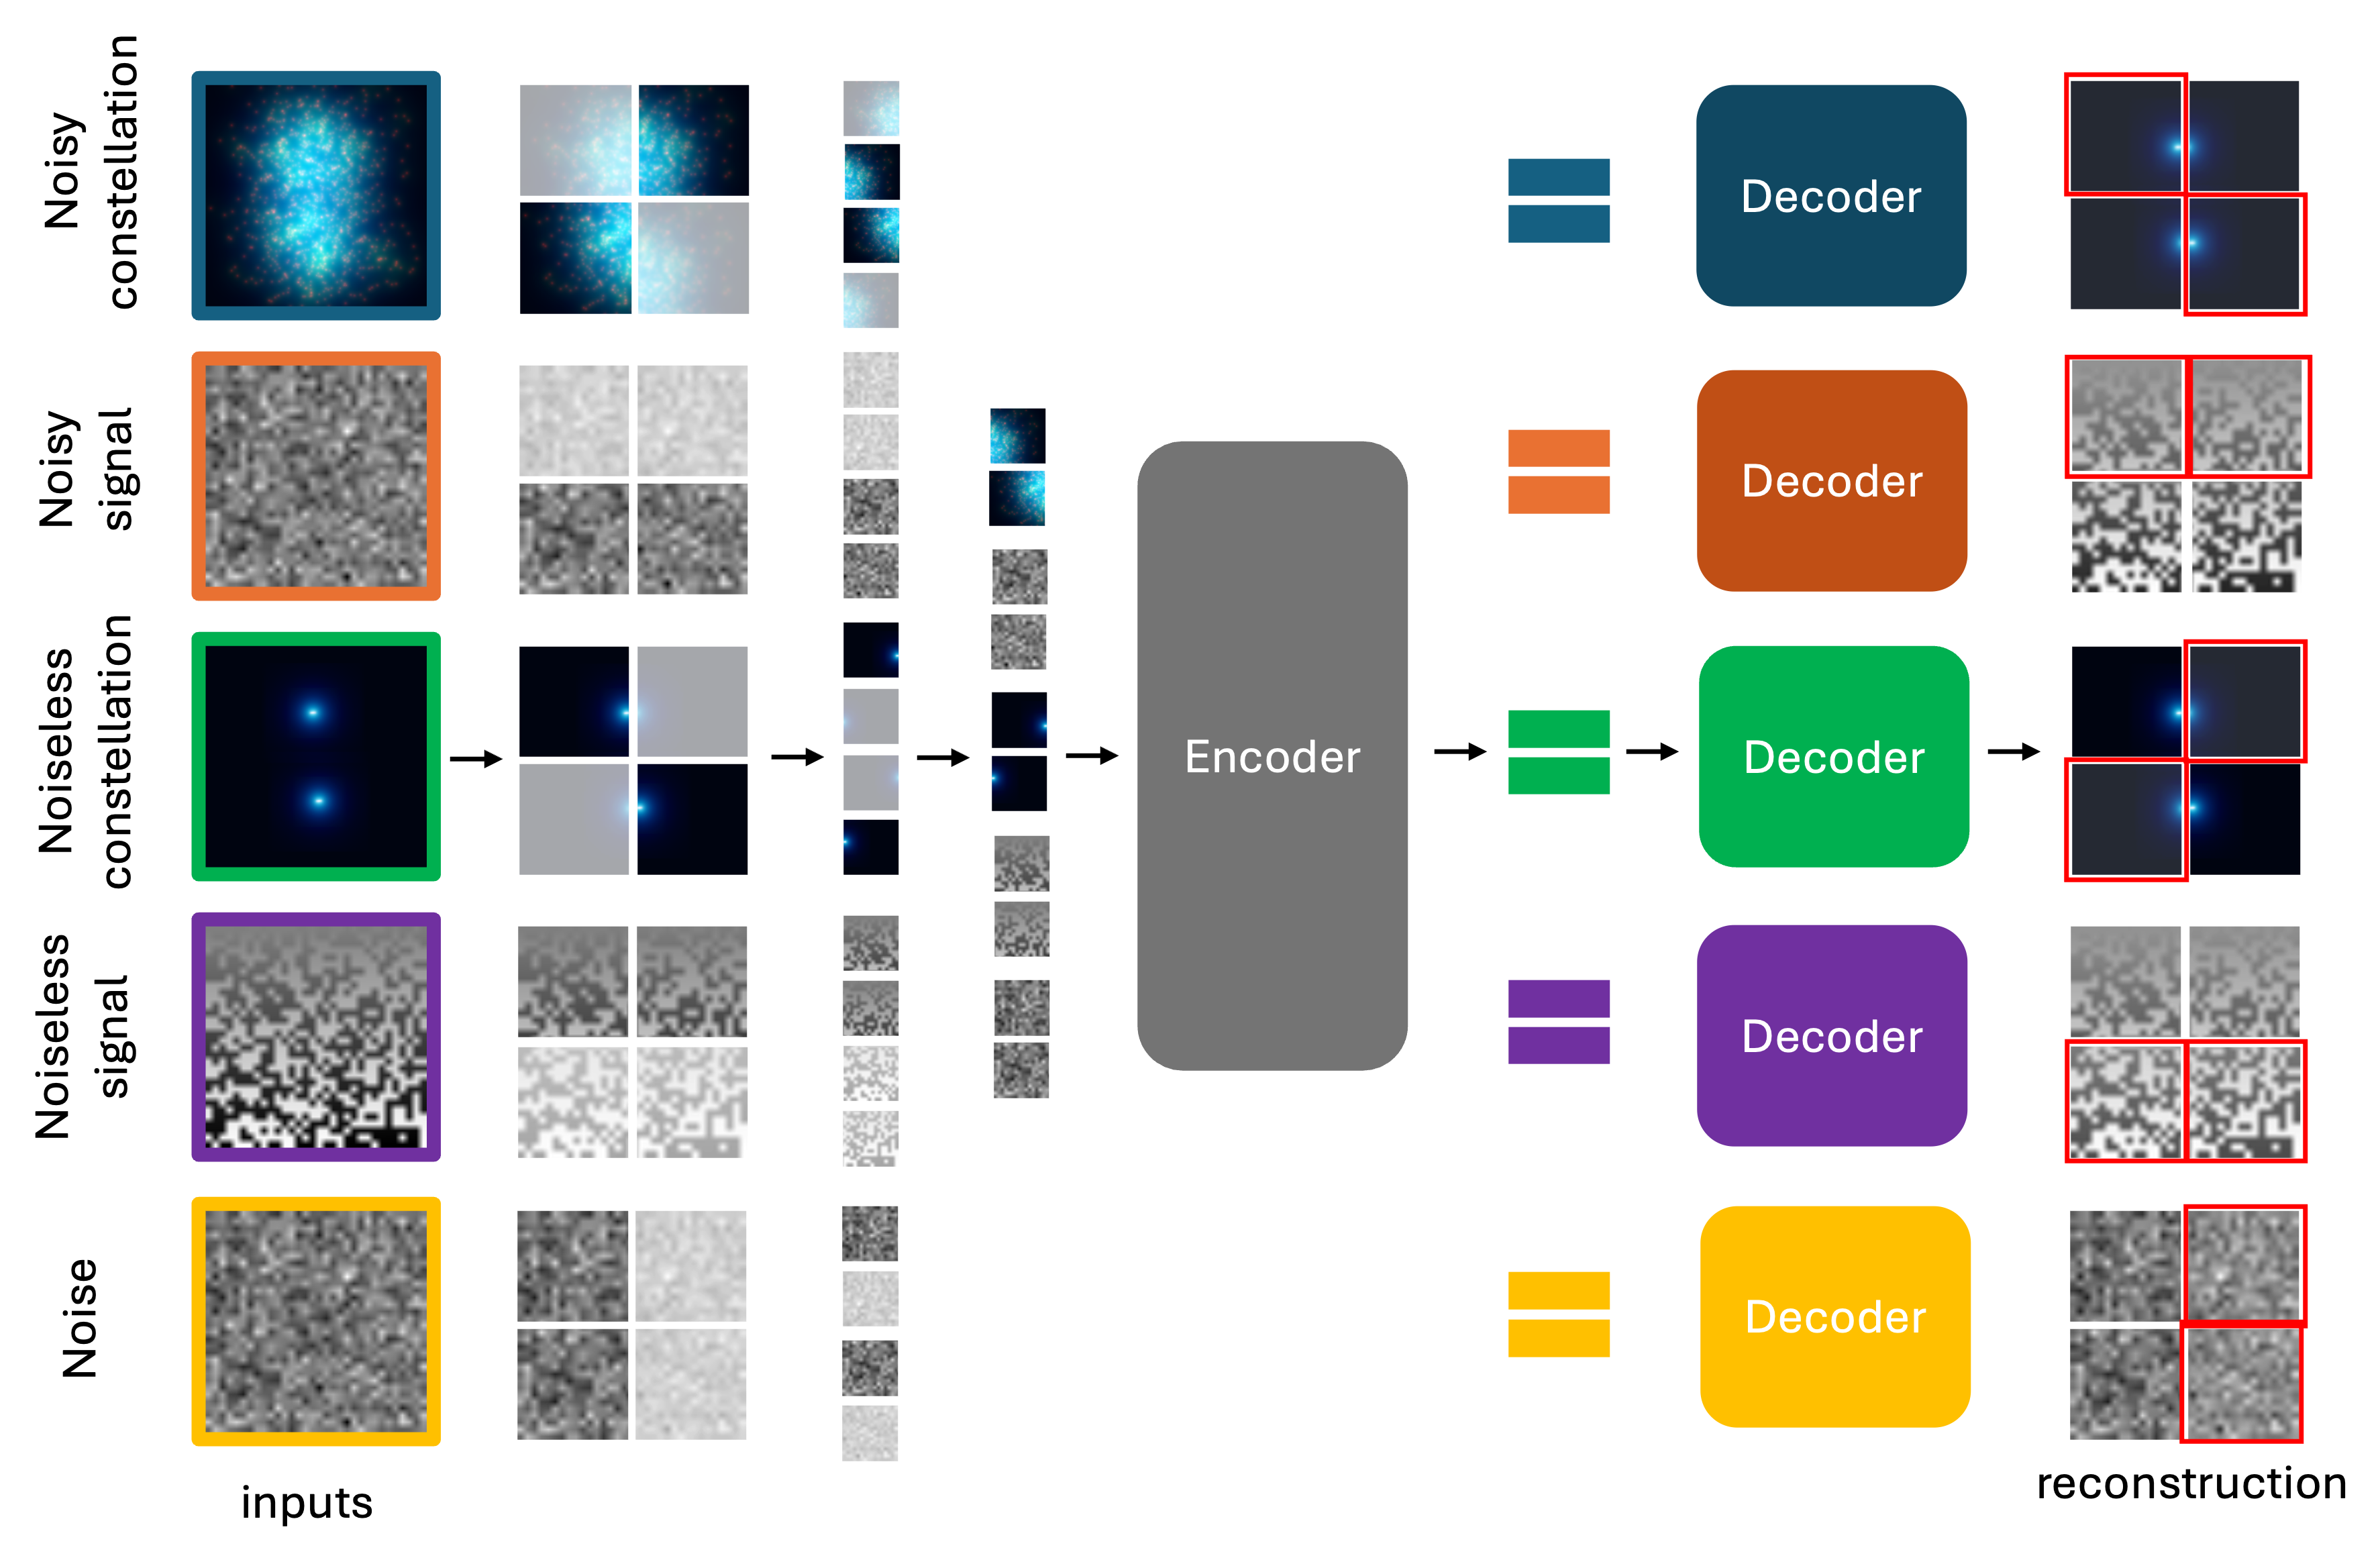
\includegraphics[width=0.9\linewidth]{FIGURES/denomae/fig.png} % Adjust width as needed
    \caption{
    \textbf{DenoMAE Pretraining Strategy}: We apply a random 75\% masking (not to scale in the illustration) across all input modalities. The remaining 25\% of visible patches are processed by a shared encoder, while each modality utilizes a dedicated decoder to reconstruct its masked patches. Only the encoder is reused for fine-tuning the downstream tasks.
    }
    \label{fig:architecture} 
\end{figure*}


\section{Introduction}

In recent years, the deep learning paradigm has shifted to address the high costs and scarcity of labeled data and the intensive data demands of supervised models. Self-supervised learning has emerged as an efficient solution, allowing models to leverage abundant raw data in pretraining. This approach drastically reduces the need for labeled data during fine-tuning while maintaining strong downstream performance \cite{balestriero2023cookbookselfsupervisedlearning}. Self-supervised methods have shown remarkable success across fields like natural language processing \cite{roberts2019exploring} and computer vision \cite{caron2021emerging, radford2021learning}, paving the way for new applications in fields with sparsely labeled data, including communications.

In communication systems, particularly wireless networks, maintaining signal integrity is crucial, yet it’s often compromised by limited data availability and varying noise levels during transmission. Estimating modulation signals becomes especially challenging as noise levels fluctuate with changing SNRs \cite{zheng2024deep}. This limitation becomes particularly problematic when models encounter previously unseen modulation types \cite{9965389}. While existing models can often classify known modulation schemes, they struggle to generalize to new or noisy conditions, resulting in misclassification and necessitating extensive retraining \cite{perenda2021learning, yang2019adaptive}. This problem highlights an urgent need for robust, adaptive models that can generalize across diverse conditions with minimal reliance on labeled data.


One approach to improving generalizability and robustness is through pretraining methods that not only capture robust representations but also denoise signals effectively, enhancing classification accuracy in downstream tasks and providing scalable solutions in dynamic communication environments. Masking-based methods have traditionally been effective for denoising and improving signal clarity, but they are often limited to single-modality approaches. Though effective, these methods are inherently constrained by the information within their specific modality, which restricts their potential to leverage cross-modal interactions for more robust learning \cite{shi2023gaf, huang2022deep}. Recent advances in multimodal learning address this limitation by integrating data from multiple modalities, enhancing model robustness and enabling more flexible zero-shot learning capabilities. In works like \cite{bachmann2022multimae, bachmann20244m}, attention mechanisms and masked modeling pretraining across modalities have successfully reconstructed masked signals, proving beneficial in improving classification under complex conditions \cite{cohen2023joint, leiber2022dipencoder}.


Building on recent advancements, we adapt these techniques and present DenoMAE, a multimodal autoencoder tailored for the unique challenges in communication systems. DenoMAE's innovative approach involves treating noise as an additional modality, allowing the model to generate all other modalities from a single input modality. This unique framework helps the network gain a comprehensive understanding of noise across modalities, significantly enhancing its denoising capabilities. A random masking strategy, which hides 75\% of the input modalities, is employed to challenge the model in reconstructing the missing patches, reducing computational complexity, and introducing beneficial uncertainty conducive to effective learning.


Within the broader framework of this dissertation, DenoMAE serves as the foundational representation learning component. While Chapter~\ref{chap:plugandplay} addresses training-free classification through LLMs and Chapter~\ref{chap:meta_task} enables rapid adaptation, DenoMAE provides the robust feature encoder that learns universal signal representations from minimal labeled data. This modular approach demonstrates that wireless foundation models need not follow the massive-scale paradigm of vision and language models, but can achieve strong performance through efficient self-supervised pretraining.

Our contributions to DenoMAE are threefold:

\begin{itemize} 
\item We propose a novel multimodal paradigm that incorporates noise as an additional modality, enabling more effective pretraining on modulation signals and enhancing model resilience to noise. 
\item We demonstrate that our pre-trained model achieves significant improvements in classification accuracy under low SNR conditions, with accuracy gains of up to 22.1\% over non-pre-trained models. 
\item Our approach outperforms traditional methods, achieving superior results while requiring only one-tenth of the unlabeled data for pretraining and one-third of the labeled data for fine-tuning, underscoring its efficiency and scalability for real-world applications. 
\end{itemize}

\textbf{Framework Position and Research Questions:} Within the dissertation's modular framework for wireless foundation models, DenoMAE serves as the critical representation learning component, directly addressing \textbf{RQ1}: \textit{Can vision-based, self-supervised learning effectively transfer world knowledge to the wireless domain?} By treating wireless signals as images (constellation diagrams) and applying masked autoencoding—a technique proven successful in computer vision \cite{he2021mae}—DenoMAE demonstrates successful cross-modal knowledge transfer. The novel inclusion of noise as an explicit modality enables the encoder to learn robust, denoised representations from minimal labeled data (80\% reduction), validating that vision transformers can approximate world knowledge for wireless signals. This efficient encoder provides the feature extraction backbone that complements the LLM-based reasoning engine (Chapter~\ref{chap:plugandplay}) and enables the rapid adaptation mechanisms of Meta-Task (Chapter~\ref{chap:meta_task}). Together with CDRF's cross-modal validation (Chapter~\ref{chap:cdrf}), DenoMAE establishes that cost-effective wireless foundation models can be built through strategic modular design rather than massive isolated training.


\section{Related Work}

For a comprehensive review of modulation classification and multisensory masked modeling approaches, please refer to Chapter~\ref{chap:background}, Section~\ref{sec:related_work}. Here we briefly position our work within this landscape.

Our approach builds upon recent advances in self-supervised learning, particularly masked autoencoders (MAE) \cite{he2021mae} and multimodal learning \cite{bachmann2022multimae}. While existing methods in AMC rely on CNNs \cite{peng2017modulation}, transformers \cite{kong2023transformer}, or single-modality approaches, DenoMAE introduces a novel paradigm that treats noise as an additional modality, enabling more effective pretraining and enhanced robustness across diverse SNR conditions.


\section{Methodology}
In this work, we propose DenoMAE, an innovative pretraining method for modulation classification that leverages recent advancements in multisensory pretraining. By incorporating noise as an additional modality during pretraining, DenoMAE significantly reduces data requirements while enhancing performance in downstream classification tasks.

\begin{figure}[htbp]
    \centering
    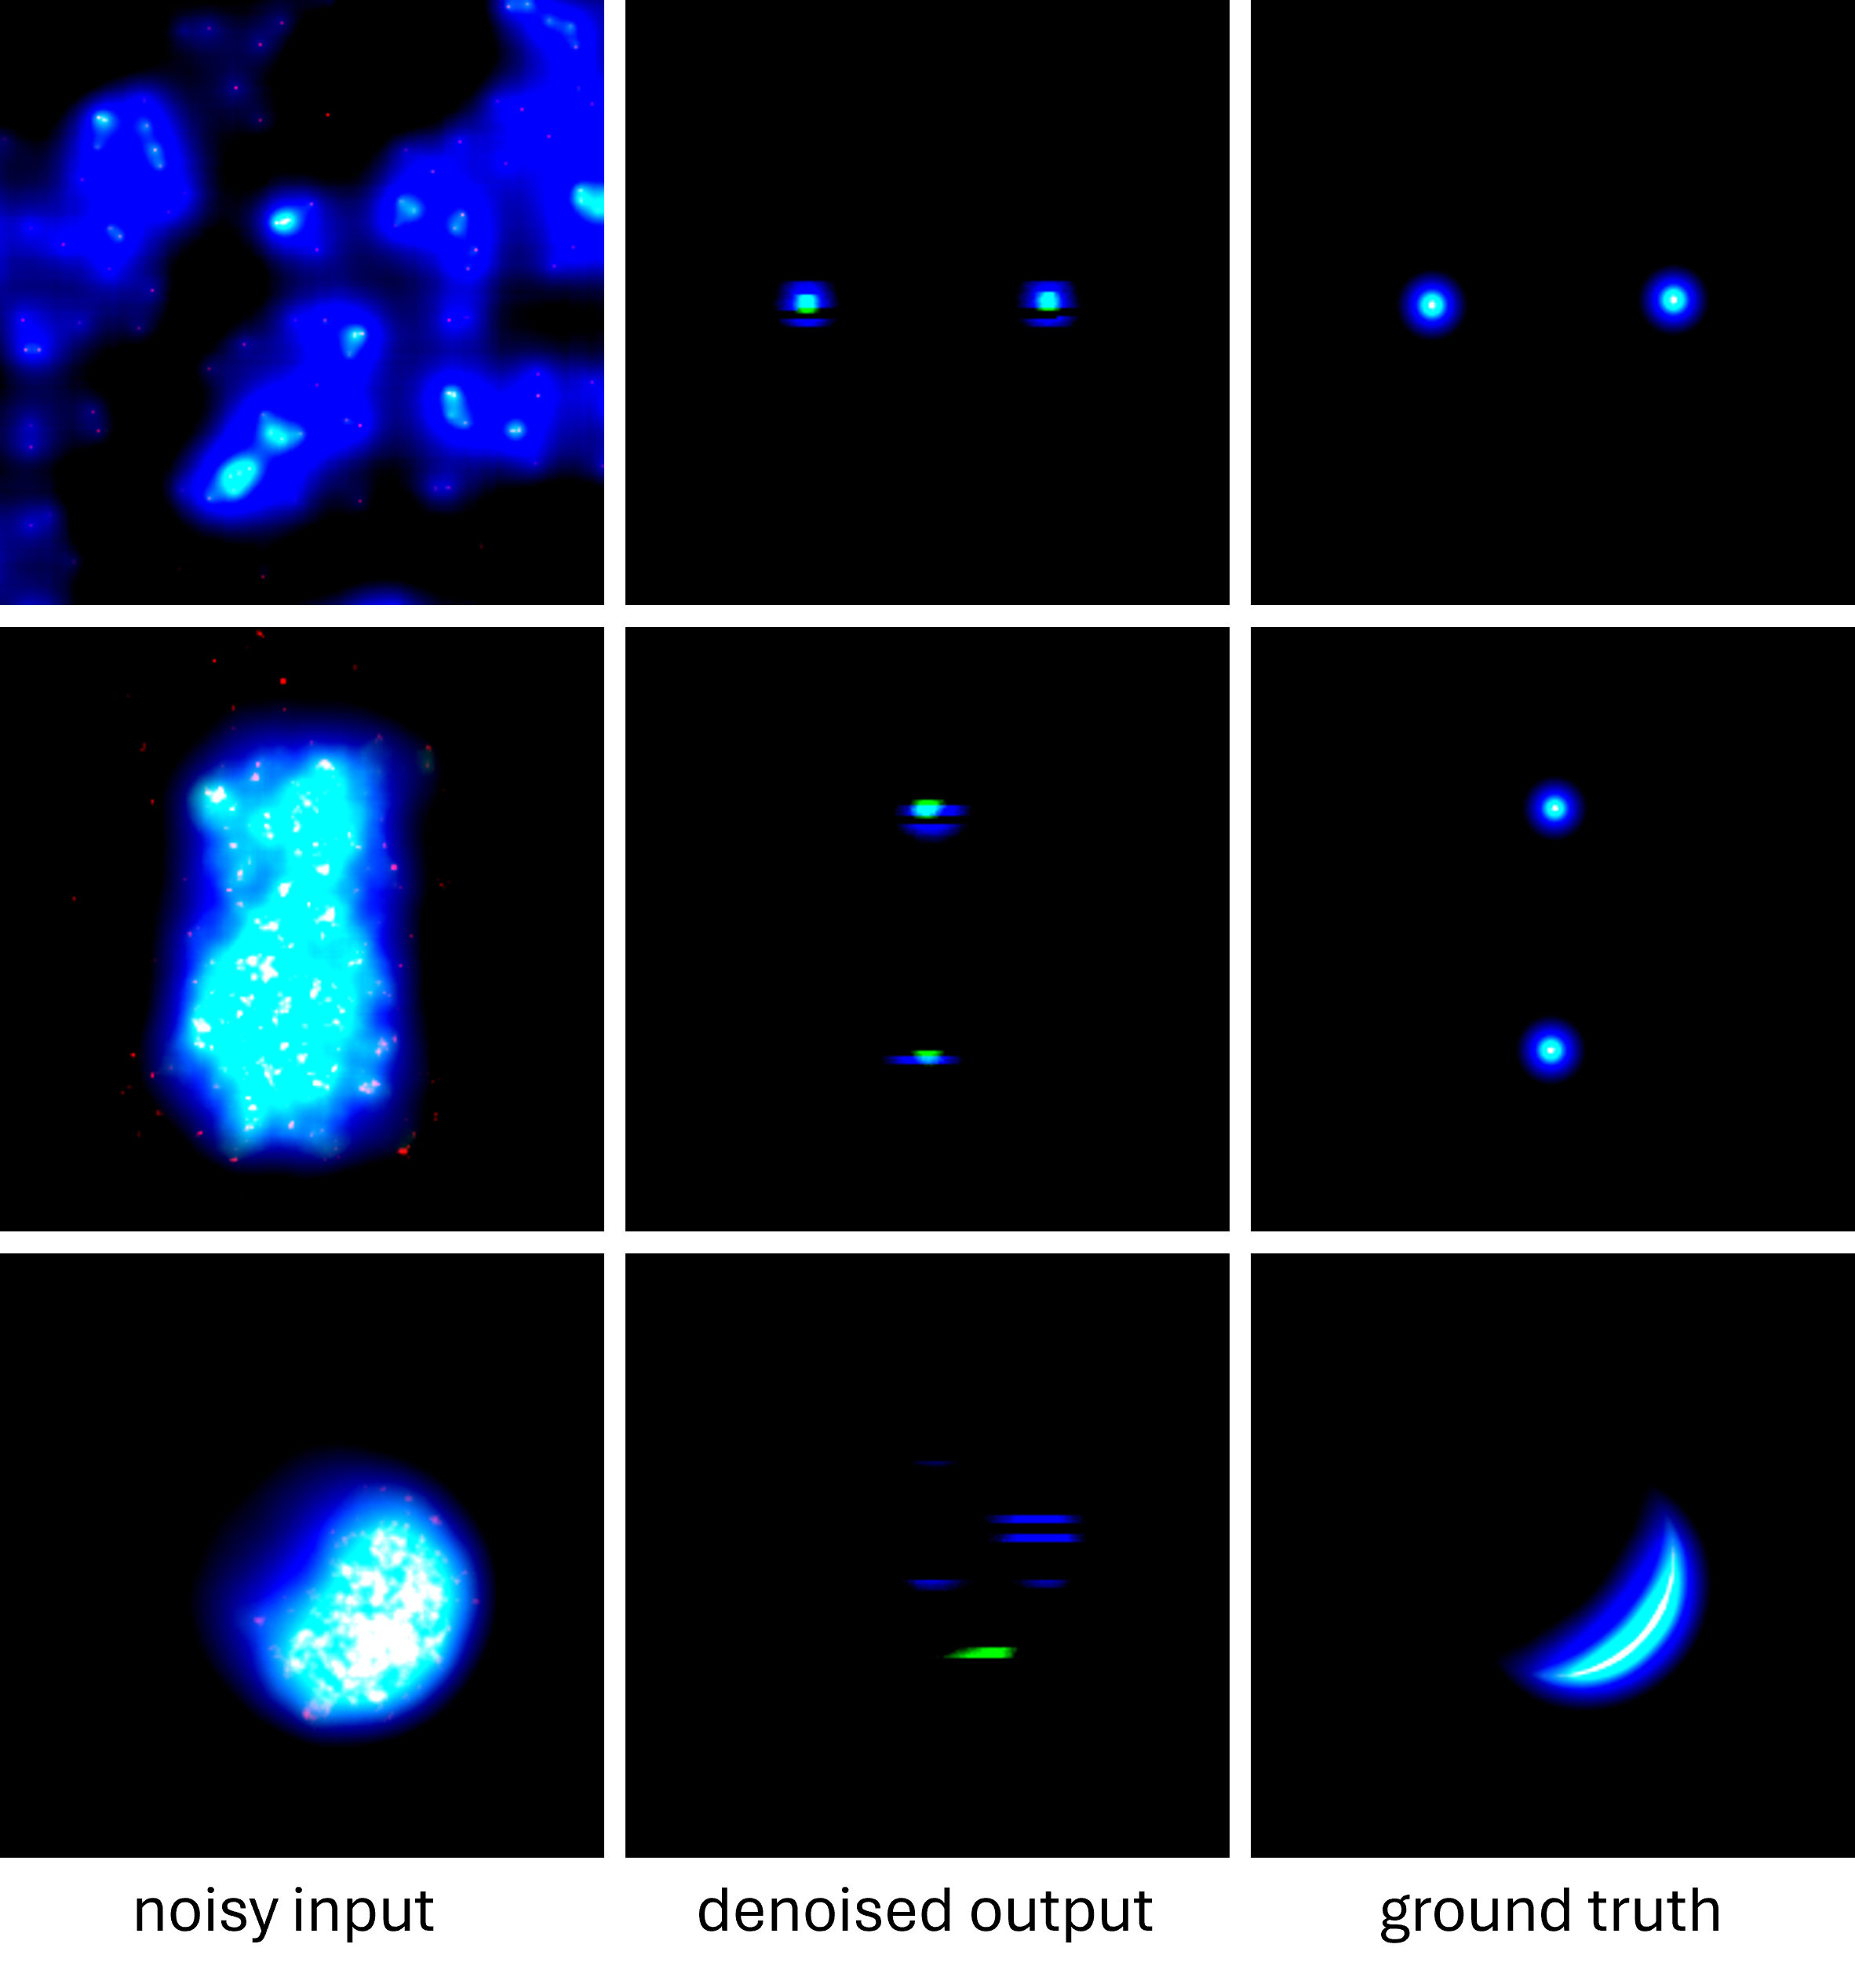
\includegraphics[width=0.9\linewidth]{FIGURES/denomae/outputs.png} % Adjust width as needed
    \caption{Denoised outputs of DenoMAE on unlabeled constellation diagrams at different SNRs during pretraining.}
    \label{fig:outputs} % Label for referencing
\end{figure}

\subsection{DenoMAE Framework}

DenoMAE consists of four primary components: input embedding, encoder, shared latent space, and decoder. Figure \ref{fig:architecture} illustrates the overall architecture.

\subsubsection{Input Embedding}

For each modality $m \in {1, ..., n}$, we represent the input as a C-channel image $X_m \in \mathbb{R}^{C \times H \times W}$. We divide each image into non-overlapping patches of size $p \times p$, resulting in $N = (H/p)^2$ patches per modality. Each patch is flattened and linearly projected to a $D$-dimensional embedding space:
$$E_m = [e^m_1, ..., e^m_N] + E_{pos}, \quad e^m_i \in \mathbb{R}^D$$
where $E_{pos}$ represents learnable positional embeddings.

\subsubsection{Encoder}

The encoder $f_{enc}$ is a series of $L$ transformer blocks. We randomly mask a high proportion (e.g., 75\%) of the input patches for each modality. The encoder processes the visible patches:
$$H_m = f_{enc}([e^m_{i_1}, ..., e^m_{i_k}]), \quad i_j \in \text{visible patches}$$

\subsubsection{Shared Latent Space}

To enable cross-modal learning, we project the encoded representations from all modalities into a shared latent space. We use a linear projection followed by layer normalization:
$$Z_m = \text{LN}(W_m H_m + b_m)$$
The shared latent representation $Z$ is the concatenation of all modality-specific projections:
$$Z = [Z_1; ...; Z_5]$$

\subsubsection{Decoder}

The decoder $f_{dec}$ reconstructs the masked patches for all modalities simultaneously. It takes the shared latent representation $Z$ as input and processes it through a series of transformer blocks. The output is then split into modality-specific representations and projected back to the original patch space:
$$\hat{X}m = f{proj_m}(f_{dec}(Z))$$
where $f_{proj_m}$ is a modality-specific projection layer.

\subsubsection{Loss Function}

We employ a multi-modal reconstruction loss that combines individual losses for each modality:
$$\mathcal{L} = \sum_{m=1}^5 w_m \mathcal{L}_m$$
where $w_m$ is the weight for modality $m$, and $\mathcal{L}_m$ is the reconstruction loss for that modality. We use the mean squared error (MSE) as the reconstruction loss:
$$\mathcal{L}m = \frac{1}{|\mathcal{M}m|} \sum{i \in \mathcal{M}m} | \hat{X}{m,i} - X{m,i} |_2^2$$


\section{Experimental Setup}
% Merge the subsections here to save space
We begin this section by detailing the parameters used for sample generation, followed by the classifier's configuration. Finally, we present the parameters applied to our downstream tasks.

\subsection{Constellation Diagram Generation}

Constellation diagrams offer a more informative approach to modulation classification compared to raw time-series signals, capturing richer detail essential for accurate interpretation \cite{doan2020learning, 9289413}. The process of generating constellation diagrams for modulation signal classification involves multiple stages. We begin by mapping modulated signals onto a $7 \times 7$ complex plane, which provides sufficient space to capture signal samples while maintaining computational efficiency for SNR ranges of -10 dB to 10 dB. The basic constellation diagram is then enhanced through a multi-step process: first, as a gray image that handles varying pixel densities where multiple samples may occupy single pixels; second, as an enhanced grayscale image that employs an exponential decay model ($B_{i,j}$) to account for both the precise position of samples within pixels and their influence on neighboring pixels. This model considers the sample point's power ($P$), the distance between sample points and pixel centroids ($d_{i,j}$), and an exponential decay rate ($\alpha$) \cite{peng2018modulation}. To make the representation compatible with DenoMAE, which expects RGB input, we generate a three-channel image by creating three distinct enhanced grayscale images from the same data samples, each utilizing different exponential decay rates. 

\subsection{Parameters in Sample Generation} %Dataset description add table

The dataset comprises signals from ten modulation formats, each originally of length $L_0 = 1024$. To conform to the transformer's input dimensions, signals undergo a two-step preprocessing: (1) reshaping to $\mathbf{S}_1 \in \mathbb{R}^{32 \times 32}$, and (2) interpolation to $\mathbf{S}2 \in \mathbb{R}^{224 \times 224}$. For formats with $L_0 > 1024$ (e.g., $L_\text{GMSK} = 8196$), signals are initially downsampled to $L_0$. To match the three-channel structure of constellation images $\mathbf{I} \in \mathbb{R}^{3 \times 224 \times 224}$, $\mathbf{S}_2$ is replicated across three channels, yielding $\mathbf{S}_3 \in \mathbb{R}^{3 \times 224 \times 224}$. All signals are sampled at $f_s = 200$ kHz, ensuring consistency across modulation formats.

\begin{figure}[htbp]
    \centering
    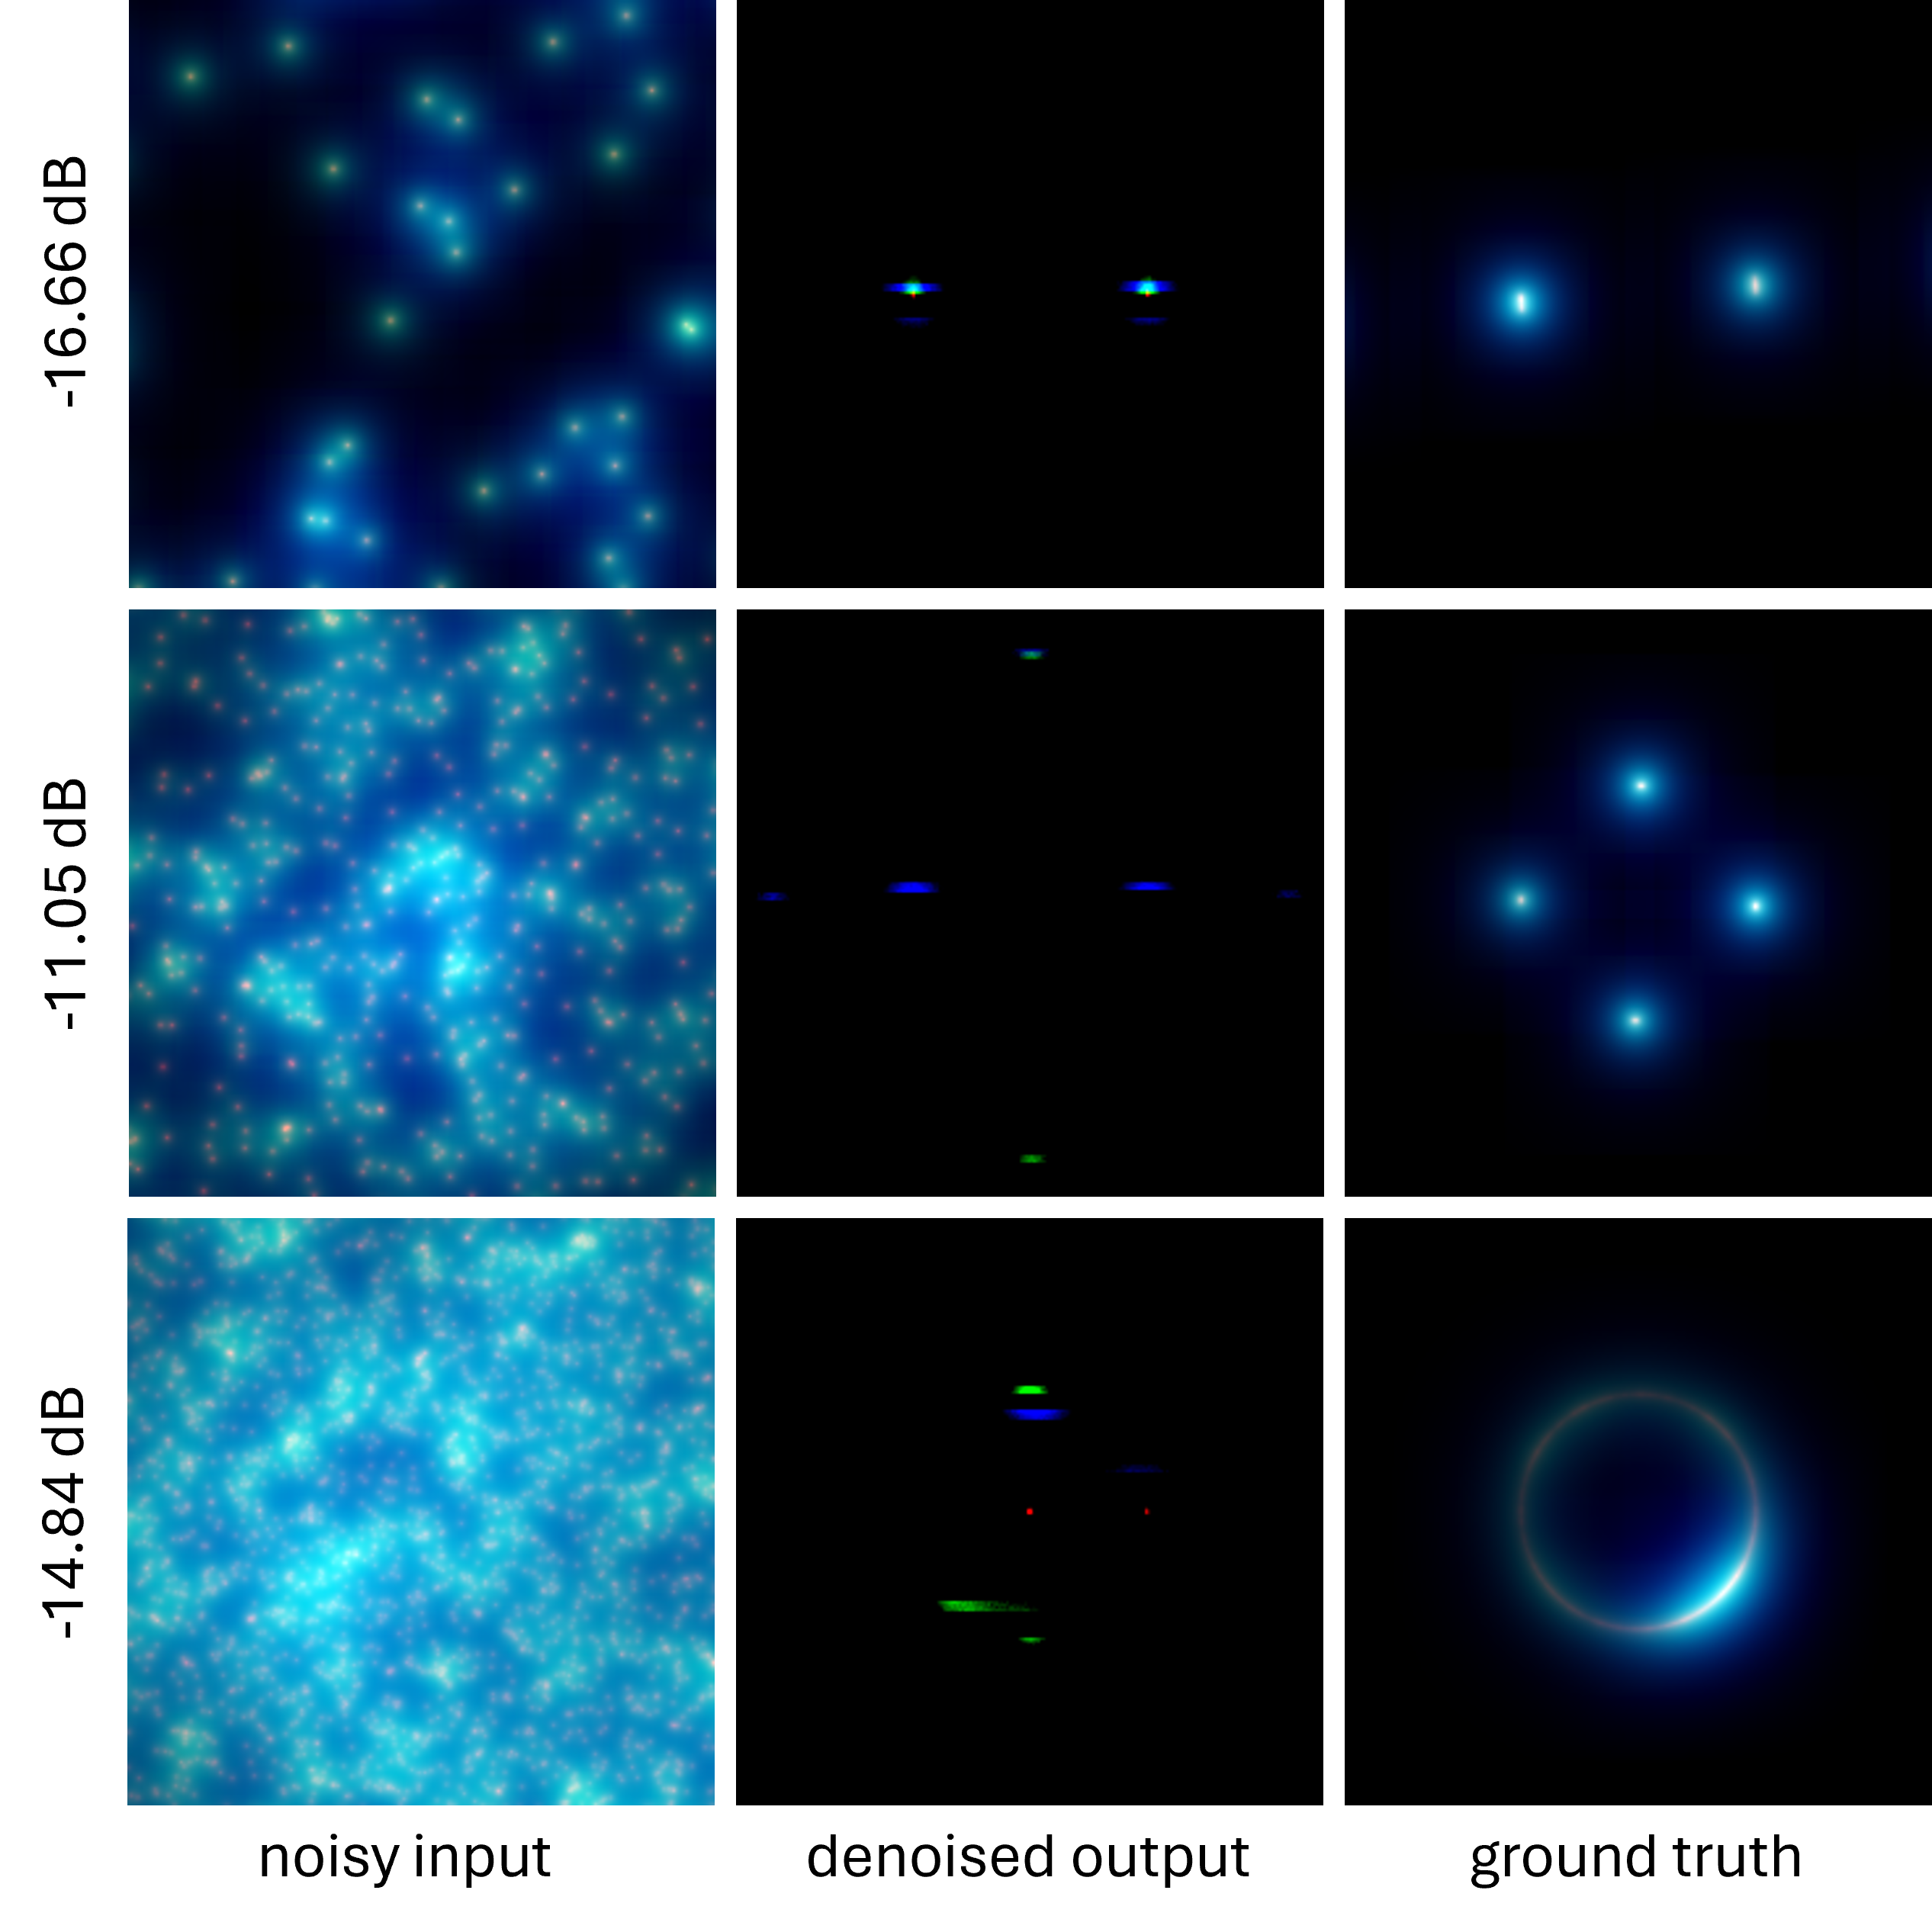
\includegraphics[width=0.9\linewidth]{FIGURES/denomae/extrapolate.png} % Adjust width as needed
    \caption{Extrapolation-ability of DenoMAE on out-of-bound much lower SNRs.}
    \label{fig:extrap} % Label for referencing
\end{figure}

\subsection{Parameters for DenoMAE}

The MultiMAE architecture processes $n$ =5 modalities of input images $\mathbf{X} \in \mathbb{R}^{3 \times 224 \times 224}$, segmented into $16 \times 16$ patches. The model employs a transformer-based encoder-decoder structure with $d_\text{model} = 768$ embedding dimensions. The encoder consists of $L_e = 12$ layers, while the decoder uses $L_d = 4$ layers, both utilizing $h = 12$ attention heads. During training, a random masking strategy with $p_\text{mask} = 0.75$ is applied. The model is optimized using AdamW with learning rate $\eta = 10^{-4}$ over $E = 100$ epochs, using batches of size $B = 64$. This flexible architecture allows for easy adaptation to various multi-modal denoising tasks.

\subsection{Finetuning Parameters}

The fine-tuning task adapts the pre-trained DenoMAE model for classification across $C = 10$ classes. The encoder $E(\cdot)$ from DenoMAE, with $d_\text{model} = 768$, is used as a backbone, followed by a classifier head $H(\cdot)$ consisting of a two-layer MLP with hidden dimension 512 and dropout $p = 0.5$. For an input $\mathbf{X} \in \mathbb{R}^{3 \times 224 \times 224}$, the model computes $\hat{y} = H(G(E(\mathbf{X})))$, where $G(\cdot)$ is global average pooling. The model is trained for $E = 150$ epochs using Adam optimizer with learning rate $\eta = 10^{-4}$ and batch size $B = 32$. Training data undergoes normalization but no augmentation.


\section{Results and Discussion}


% \begin{table*}
% \centering
% \caption{Performance Comparison Across Modalities in Downstream Task}
% \label{tab:res_table}
% \begin{tabular}{c|c|c|c|c|c|c}
% \hline
% Methods & \multicolumn{2}{c|}{Constellation} & \multicolumn{2}{c|}{Signal} & Noise & Test Accuracy (\%) \\
% \hline
%  ViT w/o pretraining & \multicolumn{2}{c|}{\checkmark }  &  \multicolumn{2}{c|}{}  &  &  74.04 \\
% \cline{2-5}
%  & Clean & Noisy & Clean & Noisy &  &  \\

% \cline{2-5} 
% \multirow{5}{*}{DenoMAE} & \checkmark &  &  &  &  & 81.30 \\
%  & \checkmark & \checkmark &  &  &  & 81.90 \\
%  & \checkmark & \checkmark & \checkmark &  &  & 83.20 \\
%  & \checkmark & \checkmark & \checkmark & \checkmark & & 83.30 \\
%  & \checkmark & \checkmark & \checkmark & \checkmark & \checkmark & 83.50 \\
% \hline
% \end{tabular}
% \end{table*}

\begin{table}
\centering
\caption{Performance Comparison Across Modalities in Downstream Task}
\label{modulations}
\begin{tabular}{c|c|c|c|c|c}
\hline
\multicolumn{2}{c|}{Constellation} & \multicolumn{2}{c|}{Signal} & Noise & Test Accuracy (\%) \\
\cline{1-4}
Clean & Noisy & Clean & Noisy &  &  \\
\hline
\cline{1-4} 
\checkmark &  &  &  &  & 81.30 \\
\checkmark & \checkmark &  &  &  & 81.90 \\
\checkmark & \checkmark & \checkmark &  &  & 83.20 \\
\checkmark & \checkmark & \checkmark & \checkmark & & 83.30 \\
\checkmark & \checkmark & \checkmark & \checkmark & \checkmark & 83.50 \\
\hline
\end{tabular}
\end{table}

This work centers on denoising and reconstructing constellation diagrams, a modality used exclusively during downstream classification tasks. In the following sections, we provide detailed insights into those findings.

\begin{figure}[htbp]
    \centering
    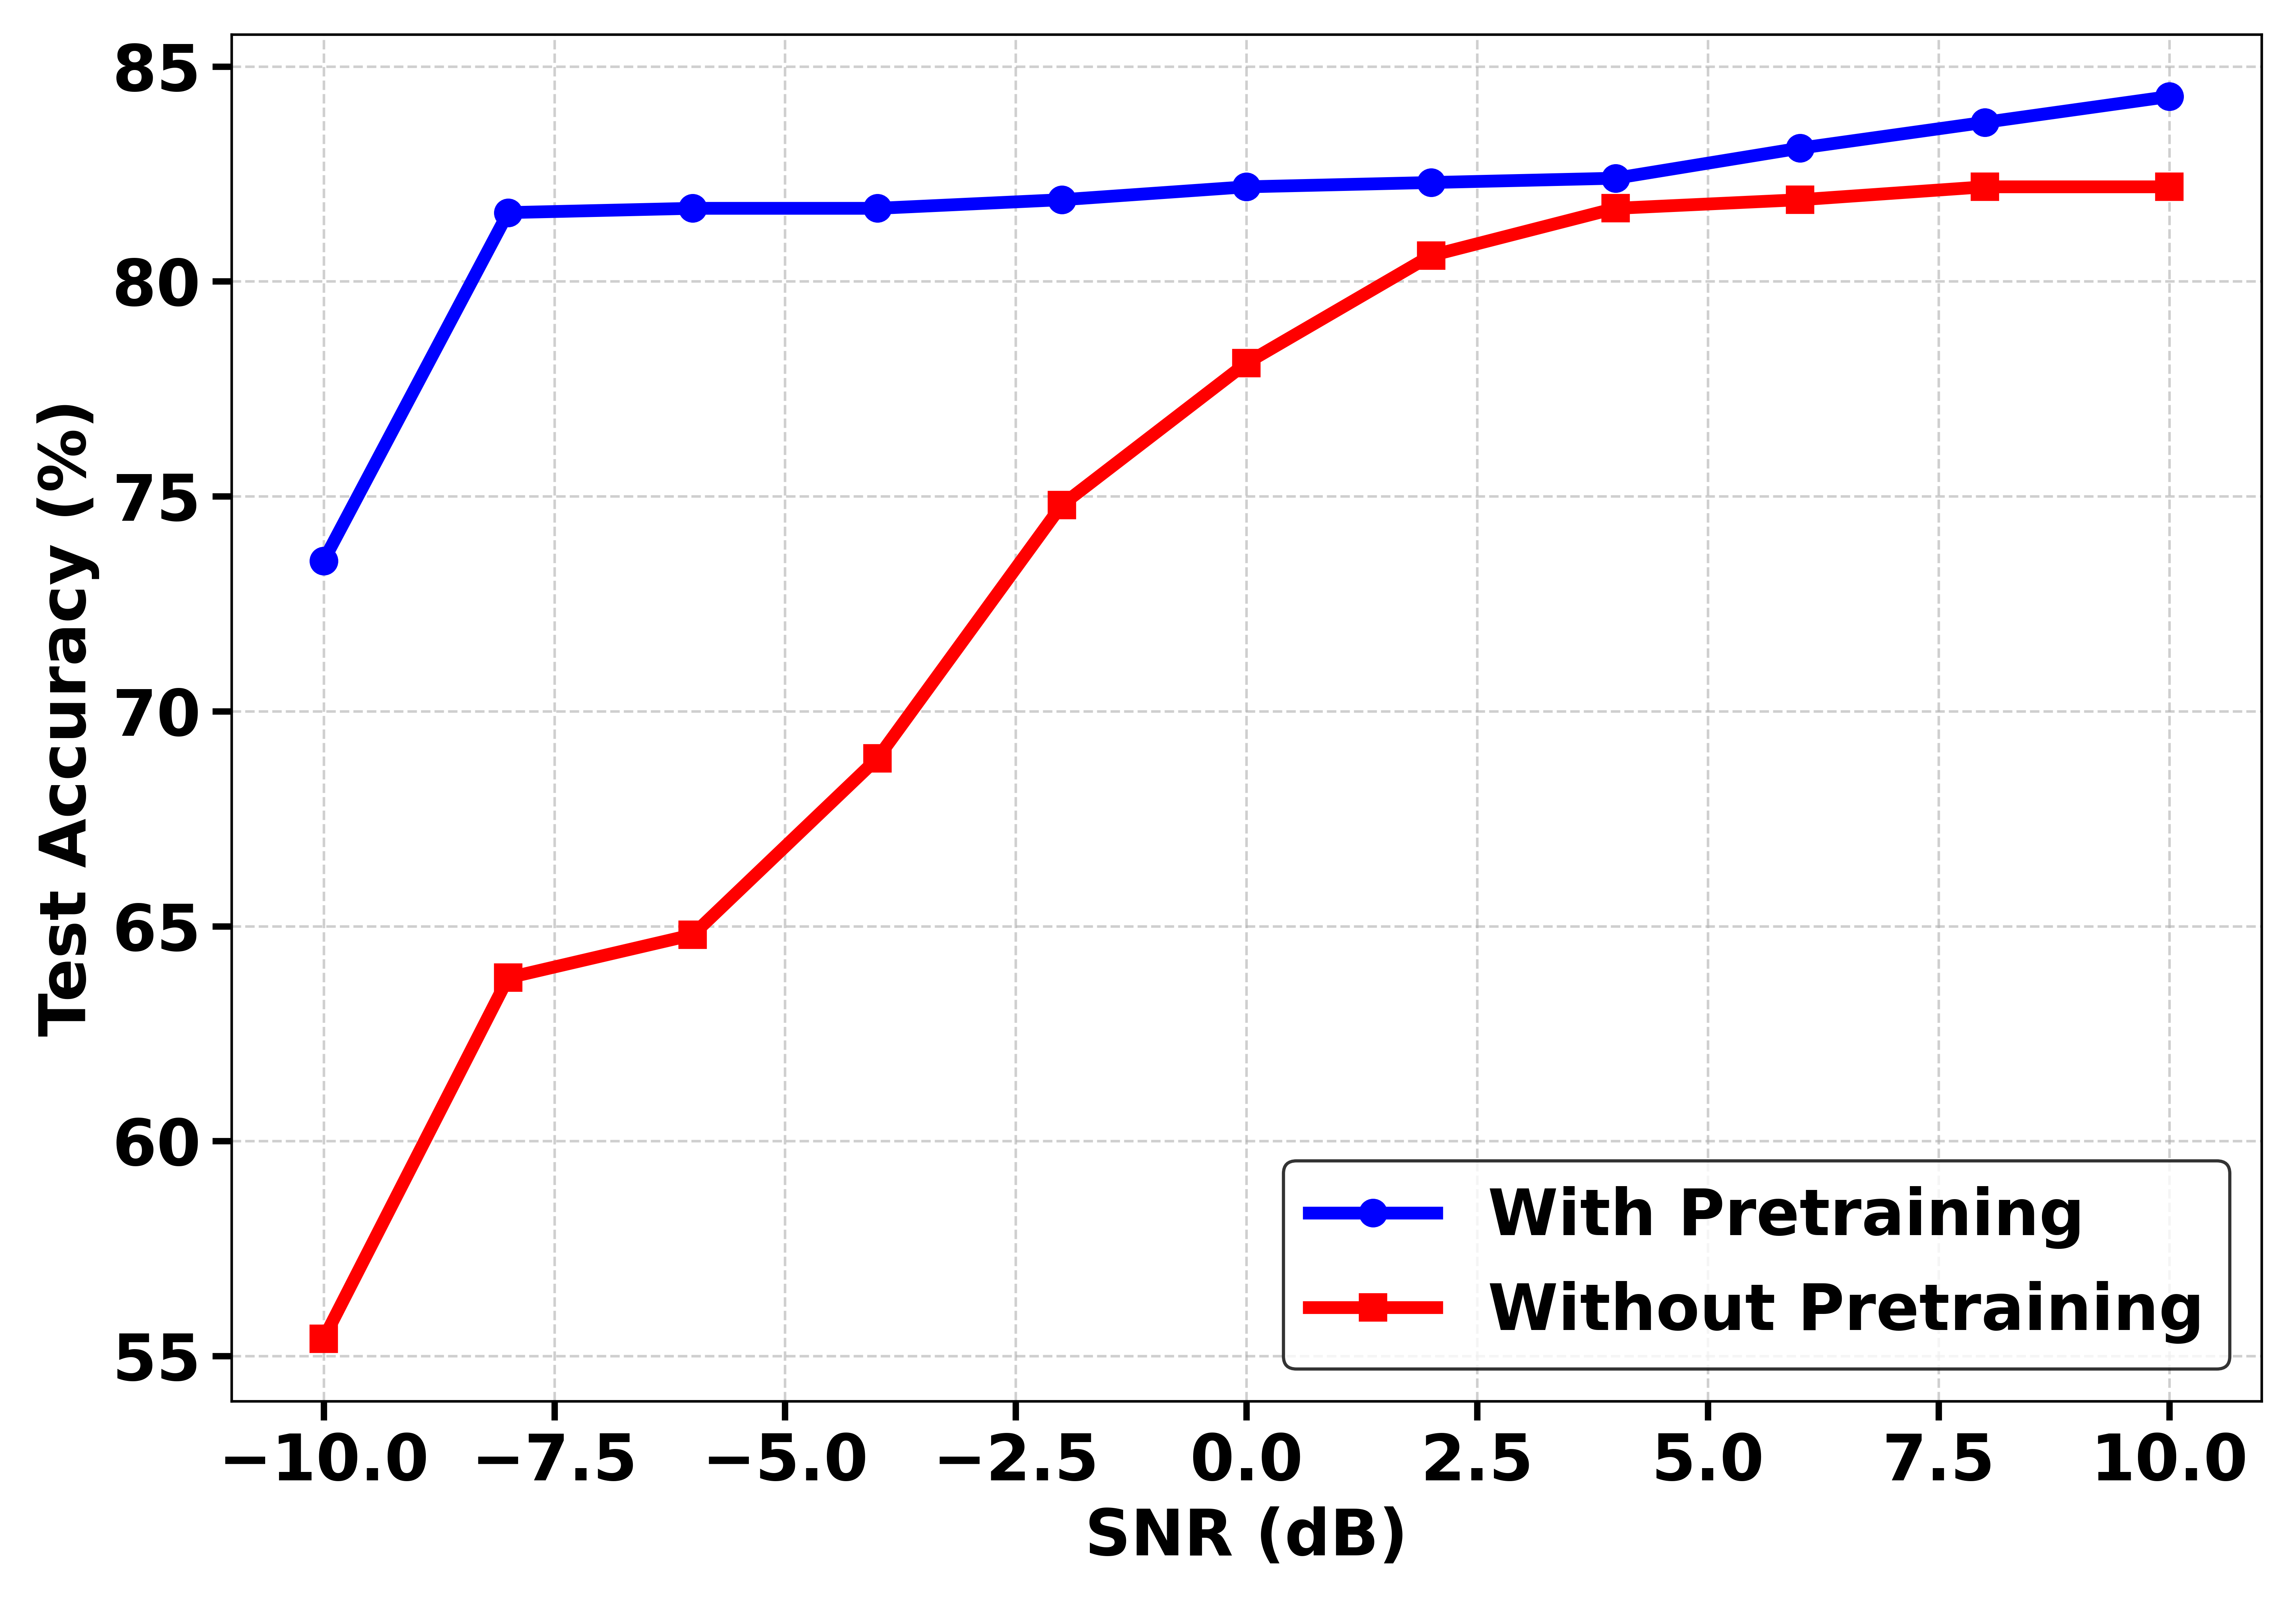
\includegraphics[width=0.9\linewidth]{FIGURES/denomae/plot.png} % Adjust width as needed
    \caption{DenoMAE fine-tuned classification accuracy for constellation diagrams at different SNRs.}
    \label{accuracy} % Label for referencing
\end{figure}



\begin{table*}[htbp]
\centering
\caption{Comparison of DenoMAE with other modulation classification methods}
\label{compare}
\begin{tabular}{cccccc}
\toprule
\multirow{2}{*}{\textbf{Methods}} & \multicolumn{2}{c}{\textbf{Number of samples}} & \multirow{2}{*}{\textbf{SNR dB}} & \multirow{2}{*}{\textbf{Number of classes}} & \multirow{2}{*}{\textbf{Test accuracy (\%)}} \\ 
\cmidrule(lr){2-3}
 & \textbf{Pretraining} & \textbf{Fine-tuning} & & \\ \midrule

AlexNet \cite{peng2018modulation}  & 800,000 (train) & 8,000 (test)  & 2 & 8 & 82.8  \\
NMformer & 106,800 & 3,000 & 0.5 - 4.5 & 10 & 71.6 \\
CNN-AMC \cite{meng2018automatic} & 79,200 & 228,060 & -6 & 4 & 50.40 \\
DL-GRF \cite{sun2022automatic} &  2,000 (train) & 200 (test) & 0 & 4 & 59 \\
DenoMAE (\textbf{Ours}) & 10,000 & 1,000 & 0.5 & 10 & 83.5 \\
DenoMAE (\textbf{Ours}) & 10,000 & 1,000 & -10 & 10 & 77.50 \\

\bottomrule
\end{tabular}
\end{table*}


% TODO: put research questions here
\subsection{Pretraining Performance}

The pretraining effectiveness of DenoMAE was evaluated using 10,000 unlabeled signal samples across five modalities. Visual inspection of the denoised constellation diagram outputs (Figure \ref{fig:outputs}) demonstrates strong reconstruction capabilities, particularly for samples in the first two rows where the model successfully removes noise while preserving signal characteristics. While reconstruction quality slightly diminishes for samples in the last row, the overall shape and pattern retention remain sufficient for downstream tasks.

\subsection{Impact of SNR}

In fine-tuning, we used 1000 labeled constellation images with 10 classes. The impact of SNR on classification performance reveals DenoMAE's robust noise resilience. As shown in Figure \ref{accuracy}, the pre-trained model achieves 77.50\% accuracy even at -10 dB SNR, with performance steadily improving to 84.30\% at 10 dB. The pretraining advantage is most pronounced in challenging low-SNR conditions, demonstrating a 22.1\% improvement over the non-pre-trained baseline at -10 dB. This performance gap gradually narrows at higher SNRs, suggesting that pretraining is particularly valuable for learning noise-robust features.


\subsection{Extrapolation on out-of-bound SNRs}

DenoMAE demonstrates impressive extrapolation capabilities when evaluated on SNR conditions significantly outside its training range. Although trained only on SNR levels above -10 dB, the model continues to deliver meaningful reconstruction performance at challenging SNR levels between -11 dB and -20 dB. As shown in Figure \ref{fig:extrap}, DenoMAE effectively denoises highly noisy input constellation diagrams, making the first two samples visually recognizable. The final sample, while impacted by extreme noise, still approximates the outer shape of the ground truth.

\subsection{Ablation Study on Modality Impact}

Our ablation study on modality impact, detailed in Table \ref{modulations}, reveals the effectiveness of the multimodal approach. The full model with five modalities (noisy image, noisy signal, noiseless image, noiseless signal, and noise) achieves 83.50\% accuracy. Performance degrades gracefully as modalities are removed, with even the single-modality version maintaining 81.30\% accuracy. This suggests that while additional modalities contribute to performance gains, the model maintains robust performance even with reduced modality input, indicating efficient cross-modal learning capabilities.

\subsection{Comparative Analysis}

% Comparative analysis against existing approaches (Table III) positions DenoMAE as a highly efficient and effective solution. Our model achieves 83.5\% accuracy using only 10,000 pretraining samples, outperforming previous methods while using significantly less data, 80x fewer samples than AlexNet, 10x fewer than NMformer, and 8x fewer than CNN-AMC. Notably, DenoMAE maintains this superior performance across 10 classes, compared to fewer classes in competing methods, demonstrating both data efficiency and broader generalization capability. These results establish DenoMAE as a state-of-the-art approach that achieves superior performance with substantially reduced data requirements while handling a more comprehensive range of modulation classes.

In Table \ref{compare}, we demonstrate the superior performance of DenoMAE against existing modulation classification approaches through comprehensive empirical evaluation. Our method achieves state-of-the-art accuracy of 83.5\% using only 10,000 pretraining and 1,000 fine-tuning samples, representing a dramatic reduction in data requirements compared to previous methods (e.g., 80× fewer samples than AlexNet, 10.7× fewer than NMformer). Notably, DenoMAE maintains robust performance across challenging SNR conditions, achieving 77.50\% accuracy even at -10 dB SNR, while handling a broader set of 10 modulation classes compared to methods like CNN-AMC and DL-GRF which only classify 4 classes. This performance significantly outpaces existing approaches, with improvements of up to 33.1\% over CNN-AMC (50.40\%) and 24.5\% over DL-GRF (59\%) under comparable or more challenging conditions, demonstrating DenoMAE's exceptional efficiency and generalization capabilities in modulation classification tasks.

\subsection{Cross-Framework Validation}

The learned representations from DenoMAE demonstrate strong transferability across the dissertation's framework. In Chapter~\ref{chap:cdrf}, we further validate DenoMAE's vision-based approach through RF drone detection, where representing signals as images enables successful transfer of computer vision models (YOLOv8, YOLOv11) to wireless tasks. This cross-validation confirms that the image-based signal representation and self-supervised pretraining strategy generalize beyond modulation classification. Additionally, the robust features learned by DenoMAE can serve as inputs to the statistical feature extraction pipeline in the Plug-and-Play LLM framework (Chapter~\ref{chap:plugandplay}), where pre-denoised constellation diagrams improve cumulant computation accuracy. The encoder's ability to learn from minimal labeled data (1,000 samples) aligns with Meta-Task's few-shot adaptation paradigm (Chapter~\ref{chap:metatask}), suggesting potential synergies in combining self-supervised pretraining with meta-learning for even greater data efficiency.


\section{Conclusion}

In this chapter, we introduced DenoMAE, a multimodal masked autoencoder that demonstrates the viability of transferring vision-based self-supervised learning techniques to the wireless domain. By representing wireless signals as images (constellation diagrams) and treating noise as an explicit modality, DenoMAE successfully answers \textbf{RQ1} affirmatively: vision transformers trained with masked autoencoding can effectively learn robust wireless signal representations through cross-modal knowledge transfer. Our extensive experiments validate three key findings: (1) the novel noise-as-modality paradigm enables superior denoising and robust feature learning, with 22.1\% accuracy improvements at -10 dB SNR; (2) multimodal learning across five modalities (clean/noisy constellation diagrams, clean/noisy time-domain signals, and noise) provides graceful performance degradation, maintaining 81.30\% accuracy even with single-modality input; (3) the approach achieves state-of-the-art performance (83.5\% accuracy across 10 classes) while requiring only 10\% of typical pretraining data and 33\% of labeled fine-tuning data, demonstrating exceptional efficiency.

\textbf{Connection to the Dissertation Framework:} DenoMAE addresses the fundamental challenge of learning robust representations with minimal labeled data, providing the encoder backbone for the modular wireless foundation model framework proposed in this dissertation. Its dramatic data efficiency (10$\times$ reduction in pretraining data, 3$\times$ reduction in labeled data) validates that strong representations can be learned economically through strategic cross-modal transfer rather than massive isolated training. This work complements the training-free reasoning capabilities of the Plug-and-Play LLM (Chapter~\ref{chap:plugandplay}), which leverages pre-trained language models to perform classification without wireless-specific training; the cross-modal validation provided by CDRF (Chapter~\ref{chap:cdrf}), which demonstrates that vision models generalize to RF drone detection; and the rapid adaptation enabled by Meta-Task (Chapter~\ref{chap:metatask}), which achieves strong performance with only 5-10 labeled examples per class. Together, these contributions demonstrate that wireless foundation models can be built through modular, cost-effective components—each approximating and integrating world knowledge from different domains—rather than requiring massive-scale end-to-end training. DenoMAE's success establishes the feasibility of the representation learning component, proving that vision-based self-supervised learning can serve as an effective pathway for economical wireless AI systems.
